\subsection {Introduction}
%\addcontentsline{toc}{section}{Introduction}

% GESIS & mission
% WTS & mission
% information extraction at WTS
% RCC
% stage 1 feedback 
% stage 2 approach and results
% remaining chapter

GESIS - the Leibniz Institute for the Social Sciences (GESIS)\footnote{\url{https://www.gesis.org/en/institute}} is the largest European research and infrastructure provider for the social sciences and offers research, data, services and infrastructures supporting all stages of the scientific process. The GESIS department \textit{Knowledge Technologies for the Social Sciences (WTS)}\footnote{\url{ https://www.gesis.org/en/institute/departments/knowledge-technologies-for-the-social-sciences/}} is responsible for developing all digital services and research data infrastructures at GESIS and aims at providing integrated access to social sciences data and services. Next to traditional social sciences research data, such as surveys and census data, an emerging focus is data infrastructures able to exploit novel forms of social sciences research data, such as large Web crawls and archives. 

Research at WTS\footnote{\url{https://www.gesis.org/en/research/applied-computer-science/labs/wts-research-labs}} addresses areas such as information retrieval, information extraction & NLP, semantic technologies and human computer interaction and aims at ensuring access and use of social sciences research data along the FAIR principles, for instance, through interlinking of research data, established vocabularies and knowledge graphs and by facilitating semantic search across distinct platforms and datasets. Due to the increasing importance of Web- and W3C standards as well as Web-based research data platforms, in addition to traditional research data portals, findability and interoperability of research data across the Web constitutes one current challenge. In the context of Web-scale reuse of social sciences resources, the extraction of structured data about scholarly entities such as datasets and methods from unstructured and semi-structured text, as found in scientific publications or resource metadata, is crucial in order to be able to uniquely identify social sciences resources and to understand their inherent relations. 

% prior work: scientifically (disambiguation, extraction, publications, web) etc tools (GESIS datasearch, GWS etc)
Prior works at WTS/GESIS addressing such challenges apply NLP and machine learning techniques to, for instance, extract and disambiguate mentions of datasets\footnote{\url{https://www.gesis.org/en/research/external-funding-projects/archive/infolis-i-and-ii}} \cite{boland2012identifying,ghavimi2016semi}), authors \cite{conf/cikm/Backes18, conf/jcdl/Backes18} or software tools \textbf{[add reference to katas work]} from scientific publications or to extract and fuse of scholarly data from large-scale Web crawls \cite{journals/semweb/YuGFLRD19, sahoo2015analysing}. Resulting pipelines and data are used to empower scholarly search engines such as the \textit{GESIS-wide search}\footnote{\url{search.gesis.org}}  \cite{conf/jcdl/HienertKBZM19} which provides federated search for scholarly resources (datasets, publications etc) across a range of GESIS information systems or the \textit{GESIS DataSearch} platform\footnote{\url{https://datasearch.gesis.org/}} \cite{Krmer2018ADD}, which enables search across a vast number of social sciences research datasets mined from the Web. 
%TODO other papers worth citing here?

% RCC
Given the strong overlap of our research and development profile with the recent initiatives of the Coleridge Initiative to evolve this research field through the Rich Context Competition (RCC)\footnote{\url{https://coleridgeinitiative.org/richcontextcompetition}}, we are enthusiastic about having participated in the RCC2018 and are looking forward to continuing this collaboration towards providing sound frameworks and tools which automate the process of interlinking and retrieving scientific resources.

The central tasks in the RCC are concerned with the extraction and disambiguation of mentions of datasets and research methods as well as the classification of scholarly articles into a discrete set of research fields. After the first phase, each team received feedback from the organizers of the RCC consisting of a quantitative and qualitative evaluation. Whereas quantitative results of our inital contribution throughout phase one have shown significant room for improvement, the qualitative assessement, conducted by four judges on a sample of ten documents, underlined the potential of our approach. 

%Judges are then asked to manually extract dataset mentions and calculate the overlap between their dataset extractions and the output of our algorithm.
%Other factors that judges took into consideration are specificity, uniqueness, and multiple occurrences of dataset mentions.
%As for the extraction of research methods and fields, no ground truth has been provided; these tasks were evaluated against the judges' expert knowledge.
%Similarly to the extraction of dataset mentions, specificity and uniqueness have been considered for these two tasks.

Having been among the four shortlisted submissions for the second phase of the RCC, this chapter describes our approaches, techniques, and additional data used to address all three tasks. As described in the following subsections, we decided to follow a module-based approach where either individual modules or the entire pipeline can be reused. The remaining chapter is organised as follows. The following Section~\ref{sec:overview} provides an overview of our approach, used background data and preprocessing steps, whereas Sections ~\ref{sec:dataset-extraction}, ~\ref{sec:research_method_extraction} and ~\ref{sec:field_classification} describe our approaches and results towards each of the tasks. Finally, we discuss our results in Section~\ref{sec:discussion} and provide an overview of future work in Section~\ref{sec:conclusion}.
%TODO best to add a short conclusion/future work section.



%Figure~\ref{figure:pipeline} shows an overview of modules developed  and their dependencies . Here, the upper three modules (which are in gray) describe the pre-processing steps (cf. Section~\ref{sec:prepro}).
%The lower four modules (blue) are used to generate the output in a pre-specified format. 



%\subsection{Task Definition of the RCC}
%In both competition phases the task was to submit a software package which is able to process PDF (respectively extracted raw text) on the Servers of the organizers.
%The software have to be able to extract dataset mentions, research methods and research fields from the given publication. More about the type of scientific publications can be found in Section~\ref{subsec:rcc-corpus}.
%In the first phase additional the software has to be able to link dataset mentions to a given set of around 10,000 dataset descriptions originate from ICPSR\footnote{\url{https://www.icpsr.umich.edu/icpsrweb/ICPSR/}} research data index.


%\subsubsection{Non-technical overview}

%\begin{itemize}
%    \item Usage of external data
%    \item Supervised machine learning Approaches
%    \item Problem of Training data: weak supervision
%\end{itemize}


% Literature Review


%\subsubsection{General Approach and Software Components}
%\subsection{Our Approach on a technical perspective}
%The central tasks in the RCC are the extraction of dataset mentions from text. 
%Even so, we considered the discovery of research methods and research fields important.
%To this end, we decided to follow a module-based approach. Users could choose to use each specific module solely or as parts of a data processing pipeline.
%Figure~\ref{figure:pipeline} shows an overview of modules developed  and their dependencies . Here, the upper three modules (which are in gray) describe the pre-processing steps (cf. Section~\ref{sec:prepro}).
%The lower four modules (blue) are used to generate the output in a pre-specified format. 

%The pre-processing step consists of extracting metadata and pure text from PDF documents. The extraction itself is done using the Cermine Tool\footnote{\url{https://github.com/CeON/CERMINE}} which returns a Journal Article Tag Suite\footnote{\url{https://jats.nlm.nih.gov}}(Jats) XML document. Then, in a second step,
%text, metadata and references are extracted. The output of the pre-processing is then used by the software modules responsible for tackling the individual sub-tasks, i.e., discovering research datasets (cf. Section~\ref{sec:dataset-extraction}), methods (cf. Section~\ref{section:research_method_extraction}) and fields (cf. Section~\ref{section:field_classification}).


%After pre-processing, a Named Enity Recognition module is used to find data set mentions. The training corpus and process is described in Section~\ref{sec:dataset-extraction}.

%In the next step, we combine all recognized mentions for each publication and compare these mentions to the metadata from `data_sets.json`.
%The mentions are used in an interim format which also persists the sentence of each mention. Also, all years are extracted from theses sentences
%and used in the retrieval process. After retrieving the best matching results, theses are returned in the target format for `data_set_citation.json`.

%For identifying research fields, we trained a classifier on abstracts and metadata crawled from the Social Science Open Access Repository\footnote{\url{https://www.ssoar.info}} (SSOAR). We used the OAI-API for this and the crawler is delivered in the module.
%We tried different classifiers and selected the best performing one, a [fasttext]() classifier, i.e. a neural net based approach with a high performance.


%\begin{figure}[t]
%    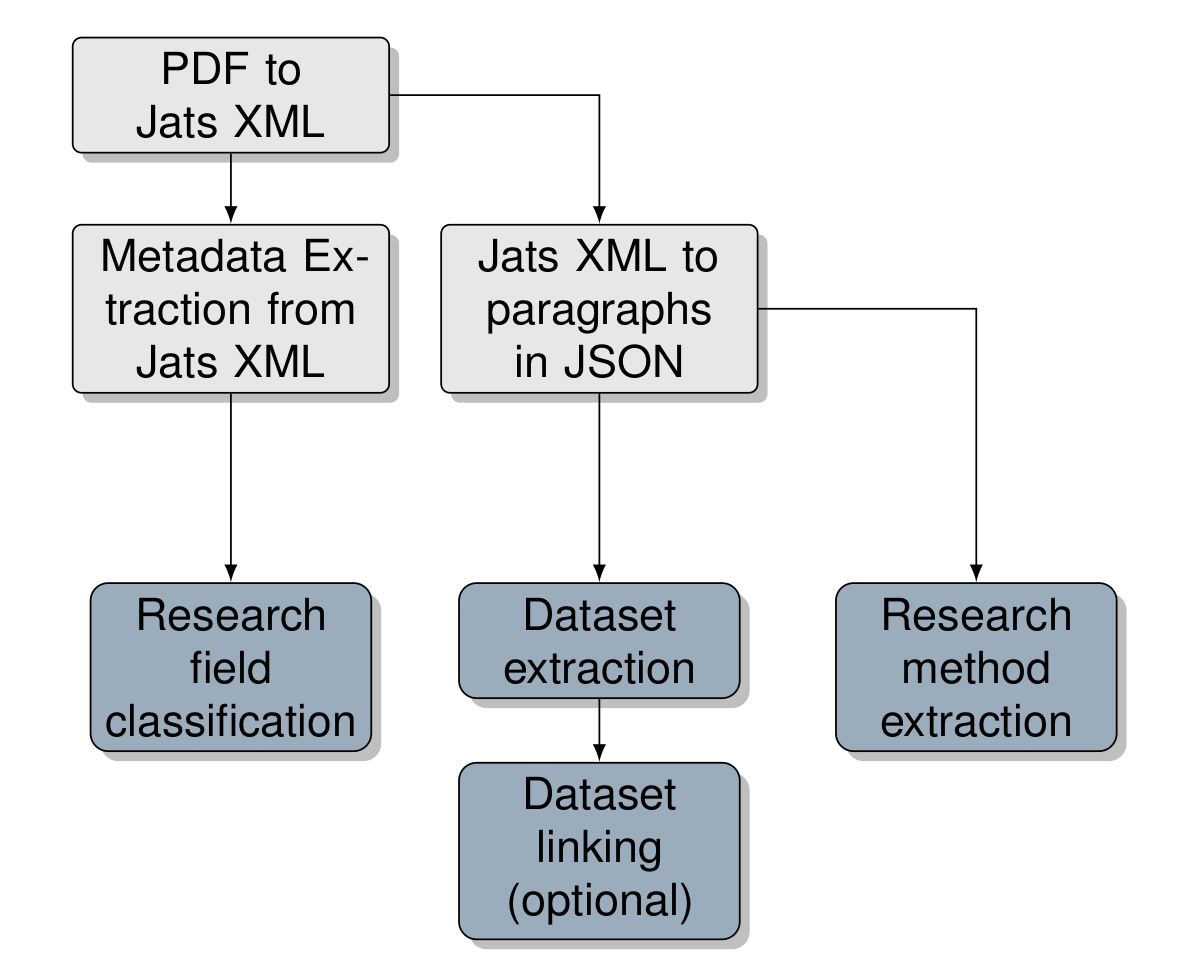
\includegraphics[width=0.47\textwidth]{figures/information-flow.png}
%    \caption{An overview of the individual software modules described in this document and their dependencies. 1- Gray: Our pre-processing pipeline. 2- Blue: three main tasks of the RCC.}
%    \label{figure:pipeline}
%\end{figure}

%\subsubsection{First Phase Feedback}
%After the first phase, each team received feedback from the organizers of the RCC.
%The feedback is two folds and consists of a quantitative and qualitative evaluation. Unfortunately, the quantitative assessment showed our algorithms did not perform well regarding precision and recall metrics. In contrast to this, our approach has been found convincing regarding the quality of results. The qualitative feedback was from a random sample of ten documents given to four judges.
%Judges are then asked to manually extract dataset mentions and calculate the overlap between their dataset extractions and the output of our algorithm.
%Other factors that judges took into consideration are specificity, uniqueness, and multiple occurrences of dataset mentions.
%As for the extraction of research methods and fields, no ground truth has been provided; these tasks were evaluated against the judges' expert knowledge.
%Similarly to the extraction of dataset mentions, specificity and uniqueness have been considered for these two tasks.
%The feedback our team received acknowledged the fact that no ground truth has been provided and our efforts regarding the extraction of research methods and fields.
%Feedback by RCC
%Section~\ref{} gives detailed overview of data provided by the RCC and additional data sources used in our approach. :o .
